\subsection{Datenmodell}\label{subsec:datenmodell}
\todo{This}


\begin{figure}[h]
    \centering
    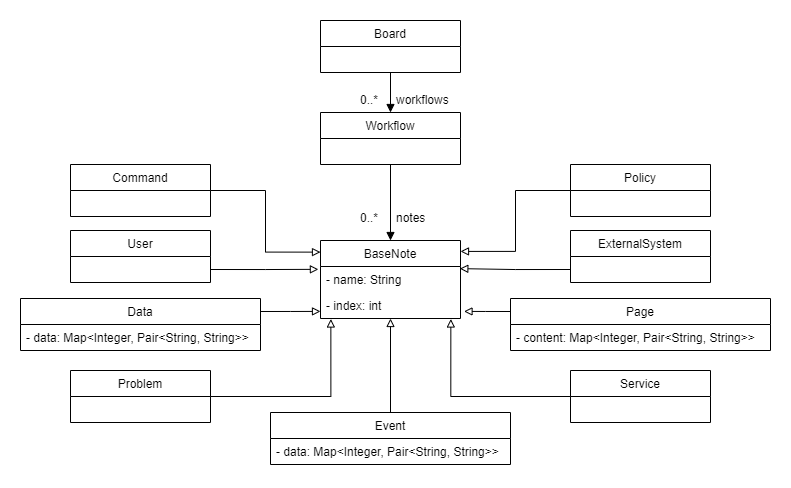
\includegraphics[width=1\textwidth]{images/3.1/classdiagram.drawio}
    \caption{Klassendiagramm fulibWorkflows}
    \label{fig:classdiagram}
\end{figure}

\todo{Rewrite the following part}

Bevor anhand eines Beispiels die Verwendung einer exit-Methode erläutert wird, ist es notwendig das Datenmodell genauer zu betrachten.
In Abbildung~\ref{fig:classdiagram} ist das Klassendiagramm abgebildet, welches die Struktur eines \ac{ES}-Boards nach dem Parsen der YAML-Eingabe widerspiegelt.
Jeder Note besitzt eine dazugehörige Klasse, welche von BaseNote erbt.
Für jeden Note existiert somit ein Name und ein Index, auf welchen im folgenden Abschnitt eingegangen wird.
Da es im Event Storming ein dazugehöriges \textit{Board} gibt, ist dies ebenfalls eine Klasse, welche alle \textit{workflows} einer Eingabe hält.
Ein Workflow besteht weiterhin aus vielen Notes.
Wie zuvor bereits erläutert, sind Data, Event und Page Sonderfälle unter den Notes, da diese weitere Daten beherbergen.
Daher haben diese Klassen ein Attribut, welches diese Daten organisiert in einer Map hält.
Hierbei wird als key der Index eines Notes verwendet und das value ist ein Pair.
Das Pair beinhaltet den Bezeichner und den dazugehörigen Wert einer zusätzlichen Property eines Notes.
